\documentclass[12pt,a4paper]{article}
\usepackage[utf8]{vietnam}
\usepackage{enumerate}
\usepackage[margin=1in]{geometry}
% \usepackage{fixltx2e} %Provide \textsubscript
\usepackage{amsmath, amssymb, amsfonts}
% \usepackage{mathptmx} %Use Times New Roman fonts but not works perfectly
\usepackage{pgfplots}

\begin{document}
\tableofcontents

\newpage
\begin{enumerate}[I/]
	\item Tìm hiểu về Cerebral Blood Flow
	    \begin{enumerate}[1/]
			\item Cerebral Blood Flow (Lưu lượng máu não)
			\begin{flushleft}
				CBF được định nghĩa là thể tích máu chảy trên một đơn vị khối lượng trong
				một đơn vị thời gian trong mô não và thường được biểu thị bằng đơn vị $ml$\ máu/($100g$\textsubscript{mô}.phút). 
				Ngoài ra, người ta có thể biểu thị CBF dưới dạng lưu lượng trên một đơn vị thể tích mô não, 
				do đó tính bằng $ml$\ máu/($100ml$\textsubscript{mô}.phút).
			\end{flushleft}
			\item Phương pháp đo lường
			\begin{flushleft}
				Phương pháp đo lưu lượng máu não trong đó bệnh nhân được 
				hít một hỗn hợp khí bao gồm chất đánh dấu có chứa $15\%\ N_2O$
			\end{flushleft}
				\begin{enumerate}[a/]
					\item Cơ sở lý thuyết
					\begin{itemize}
						\item[-] Gọi $A(t)$ là nồng độ $N_2O$ trong động mạch được đo khi máu đi vào não và $V(t)$ là nồng độ $N_2O$ trong tĩnh mạch trong máu chảy ra từ não trong tĩnh mạch cổ
						\item[-] Biểu đồ thể hiện tương quan giữa $A(t)$ và $V(t)$ như sau:
					\end{itemize}
					\begin{flushleft}
						Kí hiệu lưu lượng máu là $F$ (đơn vị $mL$/phút). Xét trong 10 phút đầu tiên
						kể từ khi hít, nếu chia khoảng $\left[0,10\right]$ thành các khoảng nhỏ hơn có độ dài bằng nhau $\Delta t$ thì 
						thể tích $N_2O$ chảy qua một điểm trong động mạch trong khoảng thời gian từ $t_{i-1} \to t_i$ xấp xỉ bằng:

						Giả sử như $F$ không đổi thì ta có thể thấy được tổng thể tích khí $N_2O$ đi vào bên trong não bộ trong khoảng $10$ phút đầu xấp xỉ là
						$$\sum_{i = 1}^{n} A(t_i)F\Delta t = F \sum_{i = 1}^{n} A(t_i) \Delta t$$
						Khi $n \to \infty$ thì ta sẽ có tổng lượng $N_2O$ được đưa vào não trong $10$ phút đầu tiên là:
						$$F \int_{0}^{10} A(t)dt$$
						Bên cạnh đó, tổng lượng $N_2O$ đi ra khỏi não cùng khoảng thời gian là:
						$$F \int_{0}^{10} V(t)dt$$
						Theo đó, tổng lượng $N_2O$ thực tế đi vào trong não $10$ phút đầu tiên trong quá trình (Kí hiệu là $Q_B(10)$):
						$$Q_B(10)=F\int_{0}^{10}\left[A(t)-V(t)\right]dt$$
						Từ đó ta có:
						$$F=\frac{Q_B(10)}{\displaystyle \int_{0}^{10}\left[A(t) - V(t)\right]dt}$$
						Trong đó $\displaystyle \int_{0}^{10}\left[A(t) - V(t)\right]dt$ có thể được tính bằng quy tắc điểm giữa trong tổng Riemann, theo đó:
						$$\displaystyle \int_{0}^{10}\left[A(t) - V(t)\right]dt = \sum_{i = 1}^{n} \left[A(t_i^*)-V(t_i^*)\right] \Delta t$$
					\end{flushleft}
					\item Ví dụ minh họa
				\end{enumerate}
	\end{enumerate}
\end{enumerate}
\newpage
	\section{Tìm hiểu về Cerebral Blood Flow}
		\subsection{Cerebral Blood Flow (Lưu lượng máu não)}
		\begin{flushleft}
			CBF được định nghĩa là thể tích máu chảy trên một đơn vị khối lượng trong
			một đơn vị thời gian trong mô não và thường được biểu thị bằng đơn vị $ml$\ máu/($100g$\textsubscript{mô}.phút). 
			Ngoài ra, người ta có thể biểu thị CBF dưới dạng lưu lượng trên một đơn vị thể tích mô não, 
			do đó tính bằng $ml$\ máu/($100ml$\textsubscript{mô}.phút).
		\end{flushleft}
		\subsection{Phương pháp đo lường}
		\begin{flushleft}
			Phương pháp đo lưu lượng máu não trong đó bệnh nhân được 
			hít một hỗn hợp khí bao gồm chất đánh dấu có chứa $15\%\ N_2O$
		\end{flushleft}
			\subsubsection{Cơ sở lý thuyết}
			\begin{itemize}
				\item[-] Gọi $A(t)$ là nồng độ $N_2O$ trong động mạch được đo khi máu đi vào não và $V(t)$ là nồng độ $N_2O$ trong tĩnh mạch trong máu chảy ra từ não trong tĩnh mạch cổ
				\item[-] Biểu đồ thể hiện tương quan giữa $A(t)$ và $V(t)$ như sau:
			\end{itemize}
			\begin{flushleft}
				Kí hiệu lưu lượng máu là $F$ (đơn vị $mL$/phút). Xét trong 10 phút đầu tiên
				kể từ khi hít, nếu chia khoảng $\left[0,10\right]$ thành các khoảng nhỏ hơn có độ dài bằng nhau $\Delta t$ thì 
				thể tích $N_2O$ chảy qua một điểm trong động mạch trong khoảng thời gian từ $t_{i-1} \to t_i$ xấp xỉ bằng:

				Giả sử như $F$ không đổi thì ta có thể thấy được tổng thể tích khí $N_2O$ đi vào bên trong não bộ trong khoảng $10$ phút đầu xấp xỉ là
				$$\sum_{i = 1}^{n} A(t_i)F\Delta t = F \sum_{i = 1}^{n} A(t_i) \Delta t$$
				Khi $n \to \infty$ thì ta sẽ có tổng lượng $N_2O$ được đưa vào não trong $10$ phút đầu tiên là:
				$$F \int_{0}^{10} A(t)dt$$
				Bên cạnh đó, tổng lượng $N_2O$ đi ra khỏi não cùng khoảng thời gian là:
				$$F \int_{0}^{10} V(t)dt$$
				Theo đó, tổng lượng $N_2O$ thực tế đi vào trong não $10$ phút đầu tiên trong quá trình (Kí hiệu là $Q_B(10)$):
				$$Q_B(10)=F\int_{0}^{10}\left[A(t)-V(t)\right]dt$$
				Từ đó ta có:
				$$F=\frac{Q_B(10)}{\displaystyle \int_{0}^{10}\left[A(t) - V(t)\right]dt}$$
				Trong đó $\displaystyle \int_{0}^{10}\left[A(t) - V(t)\right]dt$ có thể được tính bằng quy tắc điểm giữa trong tổng Riemann, theo đó:
				$$\displaystyle \int_{0}^{10}\left[A(t) - V(t)\right]dt = \sum_{i = 1}^{n} \left[A(t_i^*)-V(t_i^*)\right] \Delta t$$
			\end{flushleft}
		\subsection{Ví dụ minh họa}
\newpage
	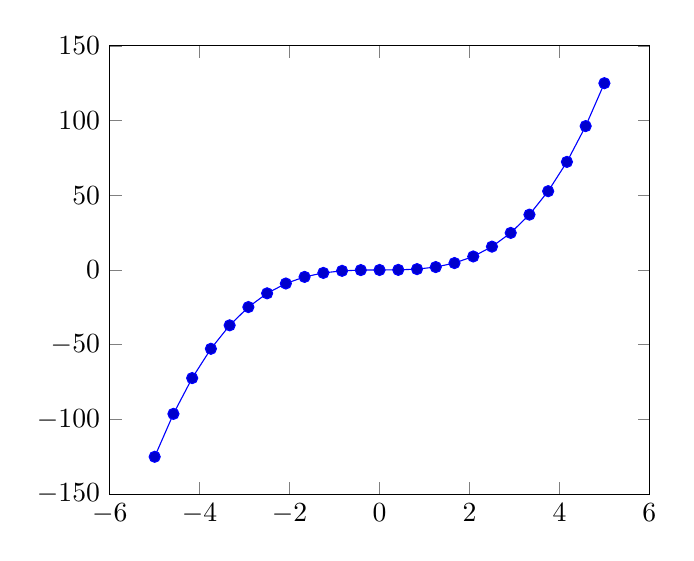
\begin{tikzpicture}
		\begin{axis}
			\addplot{x^3};
		\end{axis}
	\end{tikzpicture}
\end{document}